\documentclass{article}
\usepackage{tikz, comment}
\usepackage{pifont}
\usepackage{fontspec}
\usetikzlibrary{arrows, decorations.markings, decorations.pathreplacing}
\begin{comment}
:Title: Not defined yet
:Tags: rose;revolution;positive;periodic;period;multiple;function
:Author: Prof.Hu Ji-shan, HKUST
:Slug: No name yet

Description Here.........
\end{comment}
\begin{document}\centering

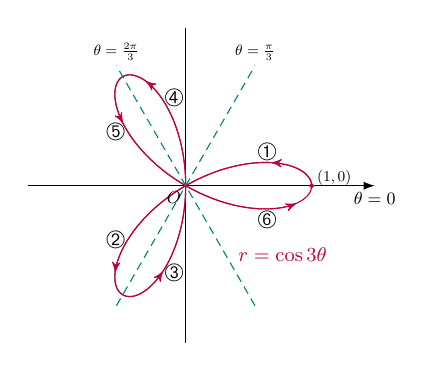
\begin{tikzpicture}[>=latex,xscale=.5*3.2, yscale=.5*3.2][font=\sf\small]

%\draw[xstep=1cm,ystep=1cm,color=gray!80] (0, -1) grid (8, 8);

\draw[->] (-1.25, 0) -- (1.5, 0)node[below, scale=0.7] {$\theta=0$};
\draw[] (0, -1.25) -- (0,1.25);

\draw[->, >=stealth', purple, samples=150, smooth, domain=0:pi/12, variable=\t]
plot ({cos(3*\t r)*cos(\t r)}, {cos(3*\t r)*sin(\t r)}) -- ({cos(3*(pi/12) r)*cos(pi/12 r)}, {cos(3*(pi/12) r)*sin(pi/12 r)});

\draw[->, >=stealth', purple, samples=150, smooth, domain=pi/12:0.885398, variable=\t]
plot ({cos(3*\t r)*cos(\t r)}, {cos(3*\t r)*sin(\t r)}) -- ({cos(3*(0.885398) r)*cos(0.885398 r)}, {cos(3*(0.885398) r)*sin(0.885398 r)});

\draw[->, >=stealth', purple, samples=150, smooth, domain=0.885398:5*pi/12, variable=\t]
plot ({cos(3*\t r)*cos(\t r)}, {cos(3*\t r)*sin(\t r)}) -- ({cos(3*(5*pi/12) r)*cos(5*pi/12 r)}, {cos(3*(5*pi/12) r)*sin(5*pi/12 r)});

\draw[->, >=stealth', purple, samples=150, smooth, domain=5*pi/12:1.9326, variable=\t]
plot ({cos(3*\t r)*cos(\t r)}, {cos(3*\t r)*sin(\t r)}) -- ({cos(3*(1.9326) r)*cos(1.9326 r)}, {cos(3*(1.9326) r)*sin(1.9326 r)});

\draw[->, >=stealth', purple, samples=150, smooth, domain=1.9326:9*pi/12, variable=\t]
plot ({cos(3*\t r)*cos(\t r)}, {cos(3*\t r)*sin(\t r)}) -- ({cos(3*(9*pi/12) r)*cos(9*pi/12 r)}, {cos(3*(9*pi/12) r)*sin(9*pi/12 r)});

\draw[->, >=stealth', purple, samples=150, smooth, domain=9*pi/12:2.97979, variable=\t]
plot ({cos(3*\t r)*cos(\t r)}, {cos(3*\t r)*sin(\t r)}) -- ({cos(3*(2.97979) r)*cos(2.97979 r)}, {cos(3*(2.97979) r)*sin(2.97979 r)});

\draw[purple, samples=150, smooth, domain=2.97979:2*pi, variable=\t]
plot ({cos(3*\t r)*cos(\t r)}, {cos(3*\t r)*sin(\t r)});

\draw[purple, fill, xscale=1/3.2, yscale=1/3.2] ({1*3.2}, {0*3.2}) circle(0.05) node[black, right, xshift=0, yshift=3, scale=0.6] {$(1, 0)$};

\node[purple, xshift=35, yshift=-25, scale=0.8] at (0,0) {$r=\cos 3\theta$};

\foreach \x in {}
\draw (\x,2pt*1.25) -- (\x,-2pt*1.25)
node[anchor=north] {}%{\tiny$\x$}
;
\foreach \x in {}
\draw (\x,2pt*1.25) -- (\x,-2pt*1.25)
node[anchor=south] {\tiny$\x$}
;
\foreach \y in {}
\draw (-2pt*1.25,\y) -- (2pt*1.25,\y)
node[anchor=east] {}%{\tiny $\y$}
;

\node at ({0.7*cos((pi/8) r)}, {0.7*sin((pi/8) r)}) {\ding{192}};
\node at ({0.7*cos((-pi/8-2*pi/3) r)}, {0.7*sin((-pi/8-2*pi/3) r)}) {\ding{193}};
\node at ({0.7*cos((pi/8-2*pi/3) r)}, {0.7*sin((pi/8-2*pi/3) r)}) {\ding{194}};
\node at ({0.7*cos((-pi/8+2*pi/3) r)}, {0.7*sin((-pi/8+2*pi/3) r)}) {\ding{195}};
\node at ({0.7*cos((pi/8+2*pi/3) r)}, {0.7*sin((pi/8+2*pi/3) r)}) {\ding{196}};
\node at ({0.7*cos((-pi/8) r)}, {0.7*sin((-pi/8) r)}) {\ding{197}};

\draw[densely dashed, teal, samples=100, smooth, domain=-0.55:0.55, variable=\x]
plot ({\x}, {tan(pi/3 r)*(\x)})node[above, black, scale=0.6] {$\theta=\frac{\pi}{3}$};

\draw[densely dashed, teal, samples=100, smooth, domain=0.55:-0.55, variable=\x]
plot ({\x}, {tan(2*pi/3 r)*(\x)})node[above, black, scale=0.6] {$\theta=\frac{2\pi}{3}$};

\node[scale=0.7] at (-0.3*1.25/4, -0.3*1.25/4) {$O$};

\end{tikzpicture}
\end{document}